\documentclass[11pt,twocolumn]{article}
\usepackage{amsmath}
\usepackage[margin=1in]{geometry}
\usepackage{graphicx}
\usepackage{import}
\usepackage{subfig}

\title{Vision-Based Autonomous Ground Vehicle Navigation}
\date{March 31, 2011}
\author{
	Michael Koval \\
	mkoval@eden.rutgers.edu \\
	Electrical and Computer Engineering
}

\begin{document}
\maketitle

\section{Introduction}
\label{sec:intro}
% 1. Overall description of IGVC
The Intelligent Ground Vehicle Competition (IGVC) is an international collegiate
robotics competition that tasks teams of undergraduate students to design,
build, and program a fully autonomous mobile ground vehicle. Specifically, the
competition consists of three distinct challenges: navigating through a winding
obstacle course, travelling between global positioning system (GPS) waypoints in
large field, and responding to messages broadcast by a Joint Architecture for
Unmanned Systems (JAUS) control system. In each of these tasks, the team has no
knowledge of the course prior to competing and navigation is further complicated
by the addition of road obstacles such as cones, barriers, switchbacks, and
potholes in the drivable regions of the course.

% 2. Alternatives to vision used by other teams
% 3. Importance of vision
Remaining in the course while autonomously navigating around these obstacles
requires that the robot has accurate knowledge of its location and objects in
its surrounding environment. Previous competitors have successfully detected
road obstacles using a combination of scanning laser range finders (LIDAR) and
stereo reconstruction. Unlike LIDAR, stereo reconstruction is capable of
providing three-dimensional data for all points in a scene, instead of only
those that are coplanar with the scanning laser rangefinder. In addition to
using stereo vision to detetct obstacles, image processing is necessary to
identify the course's painted boundaries and to locate the flags that are used
to indicate areas of safe travel.

% 4. Primary vision tasks
With the importance of computer vision clearly understood, the remainder of this
paper will discuss specific algorithms designed for use on the Navigator,
Rutgers Univeristy's entry into the 2011 Intelligent Ground Vehicle Competition.
Before discussing specific computer vision algorithms Section ~\ref{sec:robot}
describes the mechanical, sensing, and computing capabilities of the Navigator
at a high level. Making use of the onboard cameras, Section ~\ref{sec:stereo}
describes the Navigator's baseline-multiplexing stereo vision system and Section
~\ref{sec:lane} discusses monocular tracking of boundary lines. Object
recognition, such as the detection of flags and potholes, is outside the scope
of this paper and is briefly discussed as future work.

\section{Economics}
\label{sec:econ}
% ???

\section{Rutgers Navigator}
\label{sec:robot}
% 1. Brief discussion of mechanical design
% FIGURE: CAD Model and Actual Robot

\begin{figure}
	\centering
	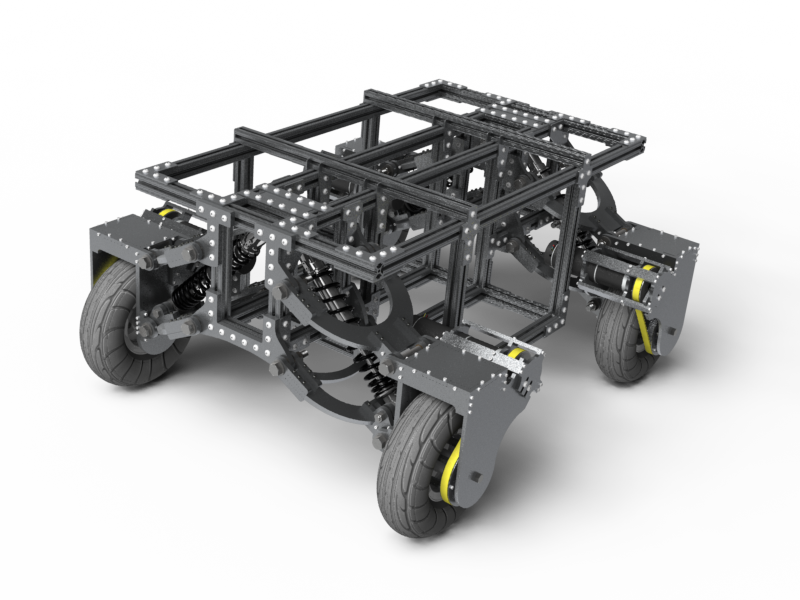
\includegraphics[width=\columnwidth]{figures/navigator-cad}
	\caption{CAD render of the Navigator.}
	\label{fig:robot-cad}
\end{figure}

% 2. Sensing capabilities
% 3. Computing capabililities and software architecture
% 4. Integration of vision with path planning (i.e. costmaps)

\section{Stereo Reconstruction}
\label{sec:stereo}
% 1. Selection of the PS3 Eye camera
Stereo vision on a mobile robot is a non-trivial problem that has traditionally
required costly hardware that support high frame rates and hardware
synchornization, such as the Bumblebee stereo vision camera. Thankfully, the
inexpensive Playstation Eye camera uses the OmniVision OV7720 capable of frame
rates up to 125 Hz and can be easily modified to support hardware
synchronization. Mounted in a custom polycarbinate case, three of these cameras
are used for stereo reconstruction.

% 2. Hardware and software camera synchronization
% FIGURE: Justification for synchronization
% FIGURE: Synchronized and desynchronized osilloscope output
% FIGURE: Synchronized and desynchronized images of a clock
\subsection{Synchronization}
\label{sec:stereo-sync}
Even if the cameras used for stereo reconstruction are attached to the same
computer and set to the same frame rate, there is no guarantee that frames will
be captured simultaeously from both cameras. If the cameras are in motion (such
as being attached to a moving robot) this delay changes the effective baseline
of the stereo system and invalidates the camera calibration\footnote{Assuming a
framerate of 30 Hz and a velocity of 10 mph, the effective baseline could change
by up to 7 cm.} that was used when stationary. As the change in the system's
baseline is a function of both the robot's velocity and the extent of the
desynchronization, it is impossible to compensate for its effects.

\begin{figure*}
	\centering
	\subfloat[Unsynchronized \texttt{VSYNC}]{
		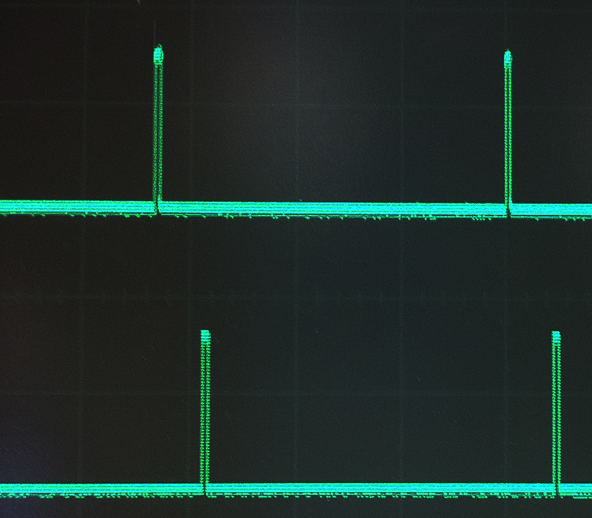
\includegraphics[width=0.24\textwidth]{figures/unsync-scope}
	}
	\subfloat[Synchronized \texttt{VSYNC}]{
		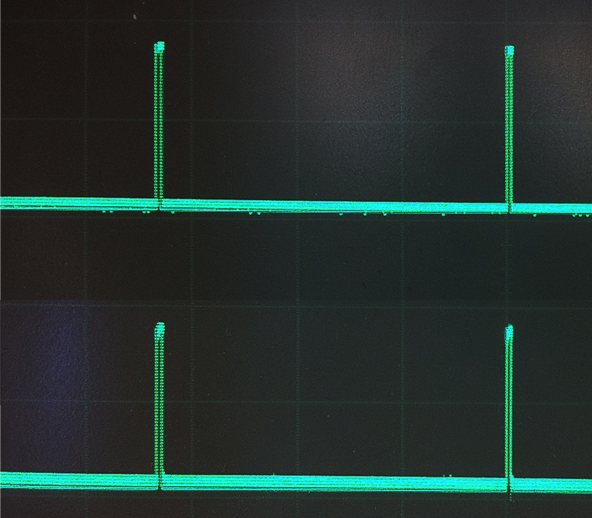
\includegraphics[width=0.24\textwidth]{figures/sync-scope}
	}
	\subfloat[Unsynchronized Frames]{
		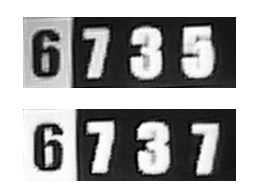
\includegraphics[width=0.24\textwidth]{figures/unsync-img}
	}
	\subfloat[Synchronized Frames]{
		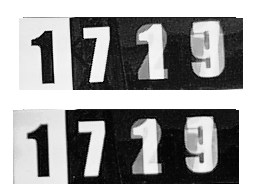
\includegraphics[width=0.24\textwidth]{figures/sync-img}
	}
	\caption{
		Verification of hardware and software camera synchronization for two
		Playstation Eye cameras. Note how only the synchronized cameras share a
		common \texttt{VSYNC} clock (left) and capture identical readings of a
		millisecond resolution timer (right).
	}
	\label{fig:stereo-sync-hard}
\end{figure*}

Hardware synchronization was achieved by  shorting the frame clock
(\texttt{VSYNC}) of the ``master'' camera to the frame trigger inputs
(\texttt{FSIN}) of the ``slave'' cameras. For electrical safety, each of the
cameras' USB grounds were shorted to force a common ground. This synchronization
guarantees that the cameras capture images simultaneously, but does not
guarantee that the images will be synchronized after the USB transfers to the
computers. Making direct use of the Video4Linux kernel module, software
synchronization was achived by fuzzy-matching of the the USB transfer
timestamps. Synchronization was verified in hardware by probing each camera's
\texttt{VSYNC} pin with an osilloscope (Figure ~\ref{fig:stereo-sync-hard}) and 
and in software by recording images of a millisecond-resolution timer (Figure
~\ref{fig:stereo-sync-soft}).

% 3. Baseline multiplexing using three cameras
% FIGURE: Effect of baseline on dead zone and maximum range.
% FIGURE: Graph of distance vs. disparity for both baselines.
\subsection{Baseline Multiplexing}
\label{sec:stereo-mux}
While unknown changes in the system's baseline is disasterous, having control
over the stereo camera's baseline can be extremely beneficial. Selecting the
best baseline is a balance of two opposing, but equally important, factors:
dead-zone and range. Decreasing the baseline shrinks the both the size of the
deadzone and the maximum range at which distances can be distinguished. This
maximum range exists because disparity is measured in pixels: there is no
discernable difference between any disparity less than one pixel. Using the
camera's intrinsic matrix, $M_{int}$, the maximum reconstructed distance is
\begin{equation*}
\end{equation*}

Analysis of previous year's competitions and considering the 20 foot width of
the navigation course, a point cloud that is useful for navigation would need
require a deadzone no larger than 2 feet and maximum that is at least 25 feet. Using the
% TODO: Focal length analysis.
% TODO: Baseline and resolution selection.

% 5. Point correspondances: SSD BM on the CPU or SAD BM on the GPU?
% 6. Software integration and cost map generation

\section{Lane Tracking}
\label{sec:lane}
% 1. Problems with other teams' approaches
% 2. Color space transformation, ground plane assumption
% 3. Creating and using a matched pulse-width filter (!)
% 4. Non-maximal supression (!)
% 5. Model fitting?
% 6. Lane width inference?

\section{Conclusion}
\label{sec:conclusion}
% ???

\section{Future Work}
\label{sec:future}
% 1. Further analysis of GPU-accelerated stereo
% 2. Stereo and/or IMU-based ground plane detection
% 4. Use stereo depth information to mask line false positives
% 3. Basic object recognition for flags, potholes, and road obstacles
% 4. Extensive testing in a software simulation (Gazebo)

\section{Acknowledgements}
% TODO: Make this phrasing less awkward.
I would like to thank all members of the Rutgers University IEEE Student Branch
for contributing to and supporting the Navigator. In particular, I am grateful
for Professor Predrag Spasojevic for serving as our faculty advisor and Adam
Stambler, Peter Vasilnak, Cody Schafer, Elie Rosen, Phillip Quiza, and Nitish
Thatte. This project would not be possible without support from our sponsors:
Knotts Corporation, 80/20 Inc., Optima Batteries, Github, and IEEE Region 1.
This project would also not be possible without the assistance provided by
Professor Kristin Dana, Steve Orbine, and John Scafidi of the Department of
Electrical and Computer Engineering and Joe Lippencott with the Department of
Industiral and Systems Engineering.

\end{document}
